\section{Experiments}

\subsection{Repeat Experiment: Do transformers recall sentences?} \label{ex:1_repeat}

Although it is known from Armeni et al. that transformers are able to do verbatim recall for lists of nouns, it is not clear that this effect translates to sentences.
In contrast with lists of arbitrary nouns, sentences are not mere enumerations of words. Instead, words in sentences follow additional structure and constraints which are available to transformers during learning and processing: sentence semantics and syntax.
For example, a transformer may have learned during training that a ``car'' frequently co-occurs with the phrase ``four wheeled vehicle'' and subsequently will assign a higher probability to the token ``car'' when probed for recall of a sentence which includes the phrase ``four wheeled vehicle''.
Second, recall of a specific sentence can stand in competition with similar syntactic structures within the training data.
Therefore, the aim of the first experiment is to determine whether the transformer is able to perform verbatim recall for sentences.

\subsubsection{Experimental Setup}
In this experiment, the encoding-sentence and test-sentence are the same sentence, whilst the control-sentences are sentences randomly sampled from the dataset.
Thus, the feature differing between the encoding-sentence and the control-sentence is verbatim repetition.
If the model is able to recall features of the encoding-sentence, then the repeat surprisal should be significantly less than $100$ percent.

Repeat surprisal is computed by taking the median surprisal value of the test-sentence\footnote{The choice of the median is due to it being less susceptible to outliers than the mean. Effectively, using the mean over the median empirically made no significant difference in any of the experiments.}.
\sloppy Formally, we use $f_\text{median}$ introduced in eq. \ref{eq:f_median} and can compute the $\texttt{repeat surprisal}_{f_\text{median}}$ with eq. \ref{eq:repeat_surprisal}.

\subsubsection{Results} \label{ex:1_repeat_results}

With an average repeat suprisal of $1.65\%$ and a median of $0.82\%$ the repeat suprisal measures for the repeat experiment floor close to $0\%$ (Figure \ref{fig:repeat_gpt2}). These results generalize across the other transformers (Figure \ref{fig:repeat_all}). Moreover, almost all repeat surprisal measures except for a few outliers fall below $5\%$.

\begin{wrapfigure}{R}[0pt]{0pt}
    \centering
    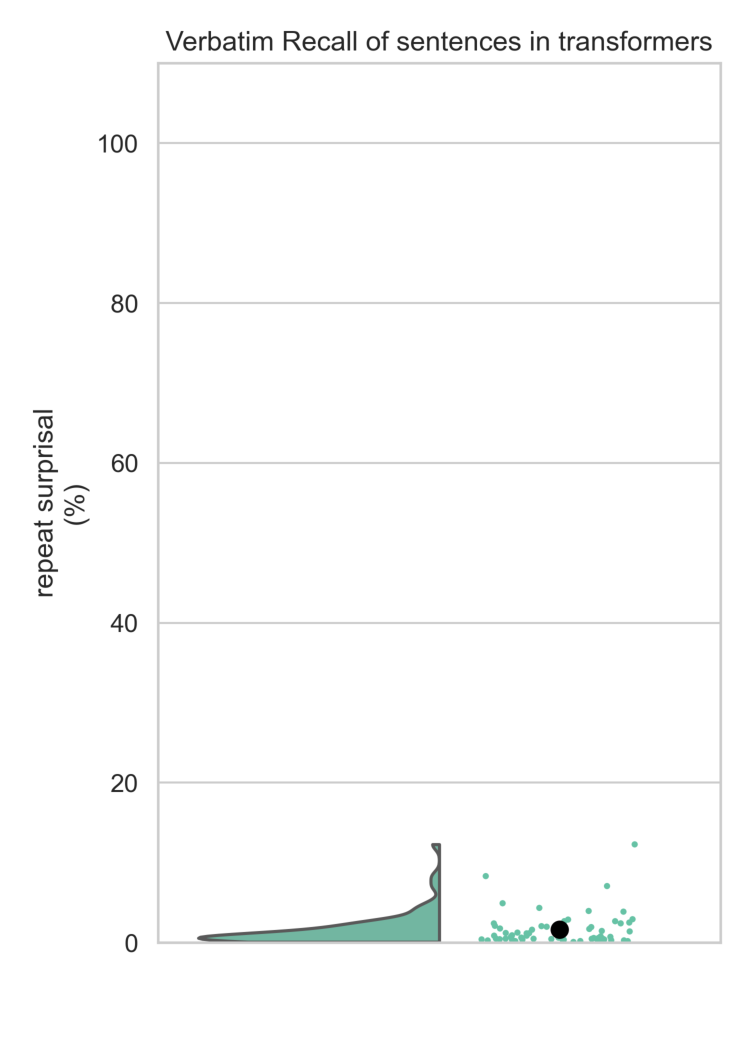
\includegraphics[width=0.5\textwidth]{experiments/repeat_surprisal_gpt2.pdf}
    \caption{Repeat surprisal of GPT-2 for verbatim repetition of sentences ($N = 60$). The Y axis shows the repeat surprisal as percentage. The ``raincloud plot'' \parencite{allen_raincloud_2019} shows the distribution of repeat surprisal as kernel density estimate (left). The points (right) are the actual repeat surprisal values for each measure. The black point (right) indicates the mean. Bootstrap $95\%$ confidence intervals are plotted around the mean, but are not visible due the consistency of the repeat surprisal in this experiment.}
    \label{fig:repeat_gpt2}
\end{wrapfigure}


\subsubsection{Interim Discussion}
The results show that transformers are able to perform verbatim recall for sentences.
This generalizes the finding that transformers can recall lists of arbitrary nouns.
Still, this experiment does not help us to differentiate between different concept-models: Any concept-model can explain this pattern of results (see \ref{app:repeat_null_explanation}).


\subsection{Word-swap experiment: Differentiating the concept-models} \label{exp:word_swap}

In order to characterize what relationships of the sentences are captured by the transformers fWM, we distinguish between four possible concept-models (see Section \ref{sec:expectations}).
In order to do that, we ran an experiment in which the results for each concept-model come apart:
In this experiment we introduce three conditions which differ by how a target word in the test sentence is swapped in the test sentence.
We then measure the repeat surprisal of that target word, and try to determine which of our concept-models best fits to our results.


\subsubsection{Experimental Setup}

We test the transformer across three conditions within our paradigm. Different from the Repeat experiment, we focus our analysis on repeat surprisal of single-tokens. The conditions only differ at the position of a verb or noun within the test-sentence of both the Test-sequence and Control-sequence.

Specifically, the first condition (\textit{repeat} - RPT) repeats the word from the encoding-sentence at the same position in the test-sentence.
The second condition (\textit{synonym} - SYN) swaps the original target word with a synonym\footnote{For details of synonym sampling see \ref{app:syn_sampling}} of the original target word.
The third condition (\textit{arbitrary} - ARB) swaps the original target word with an arbitrary word which is within the same part-of-speech (POS) category as the target-word (e.g. a noun is swapped with an arbitrary noun).

For instance, we take a measure defined by the prefix, the encoding-sentence ``A proposal to rename the species cannot be carried through.'', an intervention, and the (repeated) test-sentence ``A \textbf{proposal} to rename the species cannot be carried through.''. We mark the position of the target noun ``proposal''. Now, we measure the repeat surprisal at the position of \textbf{proposal} in the test-sentence for each condition. In RPT, proposal is repeated, in SYN proposal is swapped with a synonym (e.g. ``bid'', ``motion'', ``proposition''), and in ARB proposal is swapped with an arbitrary word within the same part-of-speech category (e.g. ``view'', ``charge'', ``microphone''). For details, see Figure \ref{fig:word_swap_setup} and \ref{app:word_swap_setup}.

Repeat surprisal is computed by selecting the surprisal value of the target noun/verb. Formally, $f_\text{sel} = \left(\left\{\left(w_1, s(w_1)\right), \dots \right\}\right) = \sum_i \delta_{w_i} s(w_i)$ where $\delta_{w_i}$ is $1$ if $w_i$ is the target word and $0$ elsewhere. We then can compute the $\texttt{repeat surprisal}_{f_\text{sel}}$ with eq. \ref{eq:repeat_surprisal}.

\subsubsection{Hypotheses} \label{sec:expectations}
Depending on which concept-model the fWM of the transformer is closer to, we expect different results across the three conditions:


\paragraph{M0: Indiscriminate}

The indiscriminate fWM increases the probabilities of previously seen words regardless of where in context they occur.
Accordingly, the target word in the Test-sequence does appear in prior context, and is assigned low surprisal values.
On the other hand, the target word in the Control-sequence in the RPT condition should be assigned a large surprisal value, as it does not appear in prior context and the transformer does not form an expectation for it.
Importantly, the repeat surprisal for target words in the RPT condition cannot be too low -- the indiscriminate WM has to distribute its probability mass over all tokens in prior context.
Subsequently, repeat surprisal values in RPT consistent with M0 are low but not $0\%$.
In the SYN and ARB conditions, an indiscriminate WM mechanism would neither expect the target word in the Test-sequence, nor in the Control-sequence (as synonyms and arbitrary tokens do not occur in context).
Hence, the repeat surprisal for ARB and SYN should be close to $100\%$.

\paragraph{M1: Plain copy-paste}
A plain copy-paste mechanism is only able to predict words which were in previous context.
In contrast to M0, under M1 the model only assigns high probabilities to one word: the exact word that followed the currently processed word.
Because the model is expecting the exact token (i.e. probability mass is concentrated on one token), repeat surprisal in RPT is expected to be $0\%$, or minimally above it.
In the SYN and ARB conditions, similarly to M0, the plain-copy-paste mechanism would neither expect the target word in the Test-sequence nor in the Control-sequence.
Hence, repeat surprisal values in ARB and SYN conditions consistent with M1 should be close to $100\%$.

\paragraph{M2: Lexical-Syntactic copy-paste}
The lexical-syntactic copy-paste mechanism allows the model to predict words within the same syntactic class.
It is expected that such a mechanism leads to repeat surprisal below $100\%$ in RPT, ARB and SYN: a repeated word RPT and a semantically similar SYN are within the same syntactic class to the original word.
Moreover, the word swap in ARB is defined over words with the same POS-category. In contrast with the plain-copy-paste mechanism where probability mass is centered on one token, the repeat surprisal in M2 should be significantly over $0\%$, as such a mechanism would distribute the probability mass over big parts of its vocabulary (e.g. all nouns).

\paragraph{M3: Word-Semantic copy-paste}
The Word-Semantic copy-paste mechanism allows for prediction of semantically similar words.
Again, such a model is expected to spread the probability mass over multiple words.
Thus, RPT is assumed to be lower than $100\%$, but not exactly $0\%$.
Furthermore, as the synonyms of the SYN condition are within the semantically similar words predicted by this model, repeat surprisal for SYN is expected be lower than $100\%$.
On the other hand, the target words in the ARB condition are very likely not semantically related to the encoding-sentence.
Hence, repeat surprisal values consistent with M3 should not be lower than $100\%$ in ARB.

\begin{figure}
    \centering
    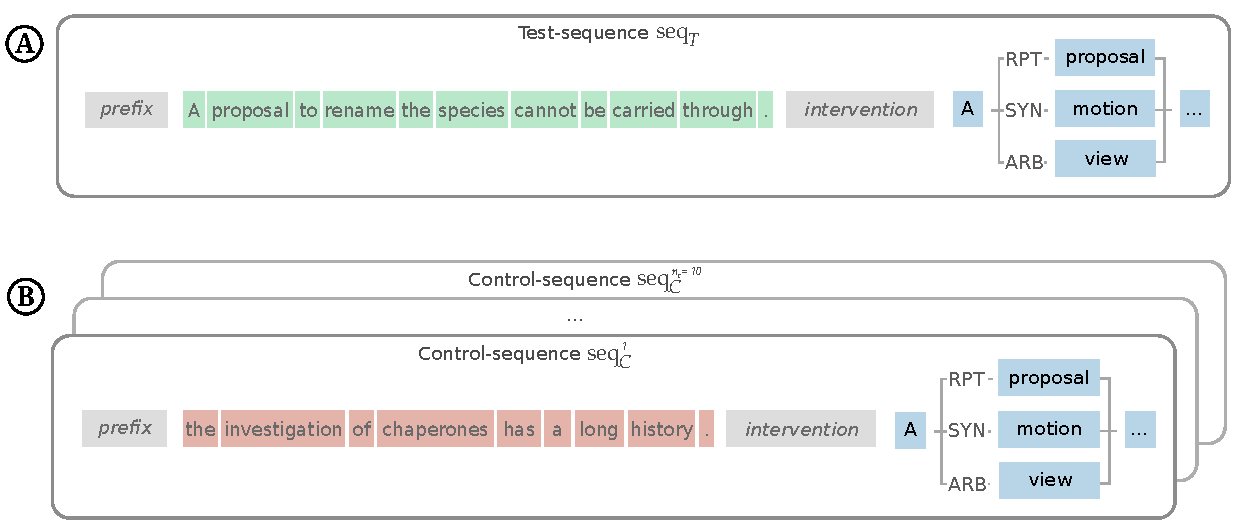
\includegraphics[width=\textwidth]{methods/word_swap_setup.pdf}
    \caption{Experimental setup for the word-swap experiment. \textbf{A}: Test-sequence for the three word swap conditions. Prefix, encoding-sentence and intervention are identical to the previous experiment. In the test-sentence, the target word ``proposal'' is either repeated (RPT), swapped with a synonym (SYN) or swapped with an arbitrary word within the same POS-category (ARB). \textbf{B}: Control-sequence for the three word swap conditions. }
    \label{fig:word_swap_setup}
\end{figure}

\subsubsection{Results}\label{ex:2_word_swap_results}

The results are visualized in Figure \ref{fig:word_swap_experiment}. Results for all transformers can be found in \ref{fig:word_swap_all}.

\paragraph{RPT}
With an average repeat surprisal for nouns of $6.8\%$ and a median of $3.1\%$ values are close to $0\%$. This means that surprisal values for the target words in the T-sequences are on average $6.8\%$ to the surprisal of target words in the C-sequences. Repeat surprisal for verbs is comparable, albeit slightly lower: the mean for verbs is $4.33\%$ and the median is $1.47\%$.

\paragraph{SYN}
The average repeat surprisal for nouns is $74.24\%$ and the median is $70.44\%$. The $95\%$ confidence interval lies well below a repeat surprisal of $100\%$. This cannot be said for verbs. With a mean of $101.14\%$ and a median of $92.21\%$ the repeat surprisal measurements are close to $100\%$. Moreover, as observable in \ref{fig:word_swap_experiment} the  $95\%$ confidence interval does not entirely lie below $100\%$.

\paragraph{ARB}
Both mean and median for verbs ($122\%$/$112.58\%$) and nouns ($128.41\%$/$120.87\%$) are well above $100\%$. This also applies to the confidence-intervals.


\begin{figure}
    \centering
    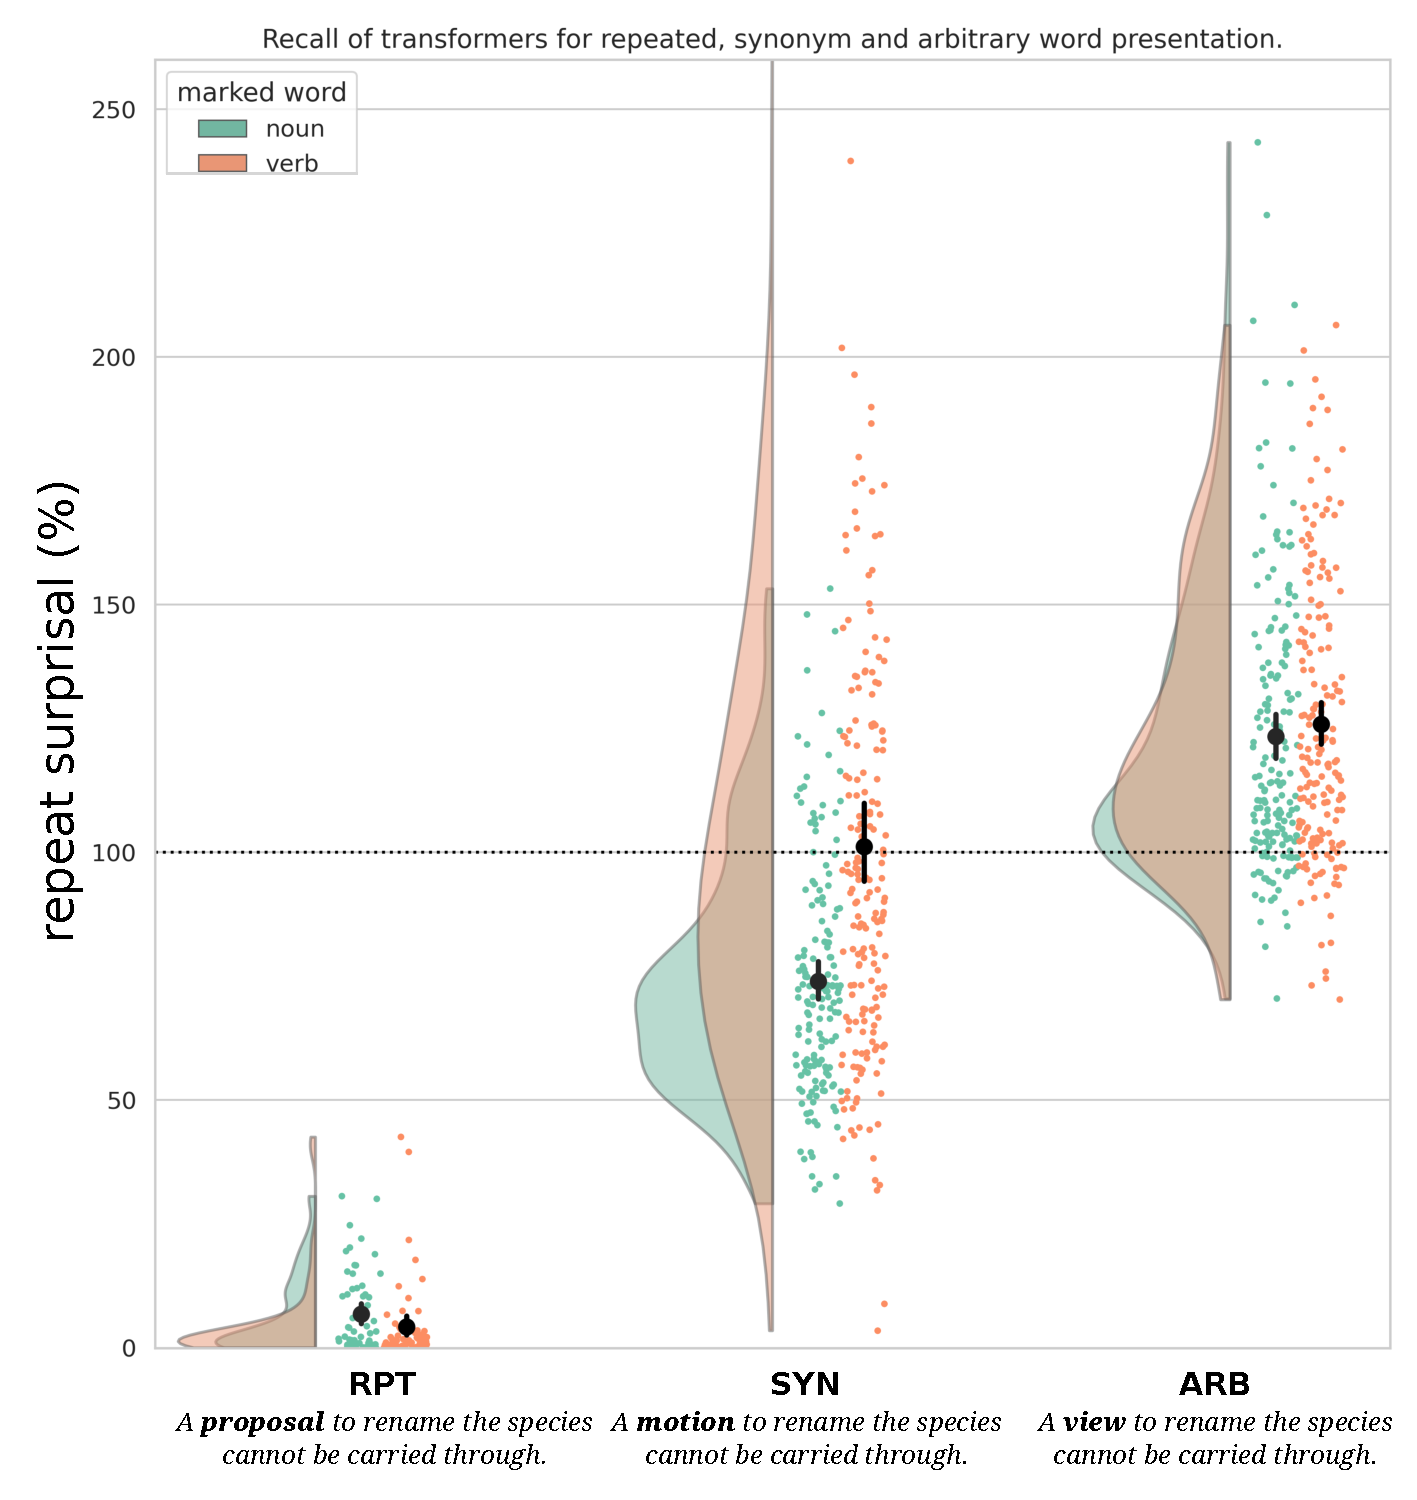
\includegraphics[width=\textwidth]{experiments/word_swap_plot.pdf}
    \caption{Raincloud plot of repeat surprisal for the RPT, SYN and ARB conditions in the word swap experiment. Given the encoding sentence "A proposal to rename the species cannot be carried through." an example test sentence with the swapped word marked is pictured below the condition labels. The results for nouns are pictured in green, the results for verbs in orange. The leftmost element shows the distributions of measurements, whilst the scatter plots show the actual repeat surprisal for every measure. The black point indicates the mean, the whiskers denote the $95\%$ confidence interval. Notice that that there are different numbers of data points per condition. Still, a clear difference between the conditions is visible.}
    \label{fig:word_swap_experiment}
\end{figure}

\subsubsection{Interim Discussion}

The word-swap experiment suggests the transformer is not employing a model such as the indiscriminate fWM M0. Although the results of the RPT condition are consistent with predictions of M0, the repeat surprisal in the ARB and SYN conditions is not centered around $100\%$.
This means the transformer is extracting information from the encoding-sentence for the prediction of tokens in the test-sentence, irrespective of the fact that the word in the test-sentence never occurred in prior context, invalidating M0.
Furthermore, the lexical-syntactic copy-paste fWM M2 also seems to be readily rejected: the results for ARB indicate that the model does not assign probabilities to all words within the same syntactic category.
On the contrary, with repeat surprisal mostly over $100\%$, the transformer is actively increasing surprisal of words within the same POS-category after the presentation of the repeated encoding-sentence.

The plain copy-paste fWM M1 seems to be a promising candidate describing the transformer fWM during sentence repetition.
The consistently low repeat surprisal values in the RPT condition strongly speak in favor of a mechanism comparable to M1.
Still, a mechanism such as M1 could not account for the results in SYN, especially not for the results regarding the nouns, as it would only predict the tokens that occur in context which is not guaranteed for synonyms.

Lastly, the word-semantic copy-paste fWM M3 seems to be most consistent with the results. The slightly reduced repeat surprisal for synonyms shows that transformers fWM indeed use the encoded information to predict semantically related words. Furthermore, it is conceivable that most of the weight is put into the verbatim repetition, as it is deemed as ``best synonym''.

We have to keep in mind the limit of this experimental design.
Since sampling of words within synonyms is not exhaustive, we may just have missed the right target words in the SYN condition on which the transformer shows a more pronounced effect.
The transformer might only have learned a subset of the targets we tested it on.
Even though this subset might not reflect human-level knowledge, it still remains relevant whether the the transformers' fWM can be characterized as a word-semantic copy-paste fWM M3 model operating on a subset synonyms.

The only condition in which results from nouns and verbs vary is the SYN condition. The result for nouns strongly speaks for the fWM of transformers being sensitive towards synonyms. On the other side, the results for verbs would suggest that the model is not sensitive at all towards synonyms for verbs. A plausible explanation for the lack of effect on verbs in SYN could be the general observation that nouns have more synonyms than verbs. Another hypothesis takes into account the placement of nouns and verbs within the sentence: whereas the median noun position within our sentences is the third position, the median verb position is the ninth. A position further along the test-sentence might lead to a stronger expectancy of the verbatim repetition, as the matched context sequence is longer. This could then result in less surprisal reduction for synonyms.

\subsection{Probability Change Analysis}\label{ex:3_prob_change_analysis}

To account for the shortcomings of the Word swap experiment, we introduce a third experiment: the probability change analysis.
Instead of analyzing the repeat surprisal on specific target words, we analyse the top six words in the transformers' output probability distribution which receive the highest change in probability after the presentation of the encoding-sentence in context.
By measuring the change of word probability given an encoding-sentence (relative to to a control-sentence) we can determine which words in the vocabulary are most influenced by the presence of the encoding-sentence.
In other words, we can have a direct look at the transformer fWM effect.
In turn, by analyzing the words that changed the most, we may determine -- in conjunction with the results from our first experiment -- which concept-model may provide the best account of fWM during sentential repetition.


\subsubsection{Experimental setup}
Similar to the word-swap experiment, the probability change analysis only focuses on the target word: a specific noun or verb within the test-sentence.
But instead of measuring the repeat surprisal of predetermined words, the probability change analysis measures the probability of all words in the vocabulary at the position of the target word in the sentence.

We first measure the output probability distribution over all words at the target word position in the Test-sequence (i.e. when the test-sentence has a relationship to the encoding-sentence in context).
We then do the same for target word position in the C-sequences (i.e. when the test-sentence has no relationship to the control-sentence in context).
We generated 10 control sequences.
We compute the average probability distribution in the 10 sequences to get an estimate of the probability for each word in the vocabulary at the target word position.

We can now measure the \textit{change in probability} between the probability distribution at the target word in the Test-sequence and the average probability distribution at the target word of the Control-sequences.
This is a direct measurement of the change in probability a transformer assigns a word when presented with a context which stands in a relationship with the test-sentence versus a context which does not stand in a relationship to the test-sentence.

The experiment was run for GPT2-base, with $60$ sentences (section \ref{met:sentences_used}).
For each sentence, the six predictions with the biggest probability change are analyzed and categorized by hand.
In total $360$ predictions were categorized both for nouns and verbs.

\begin{figure}
    \centering
    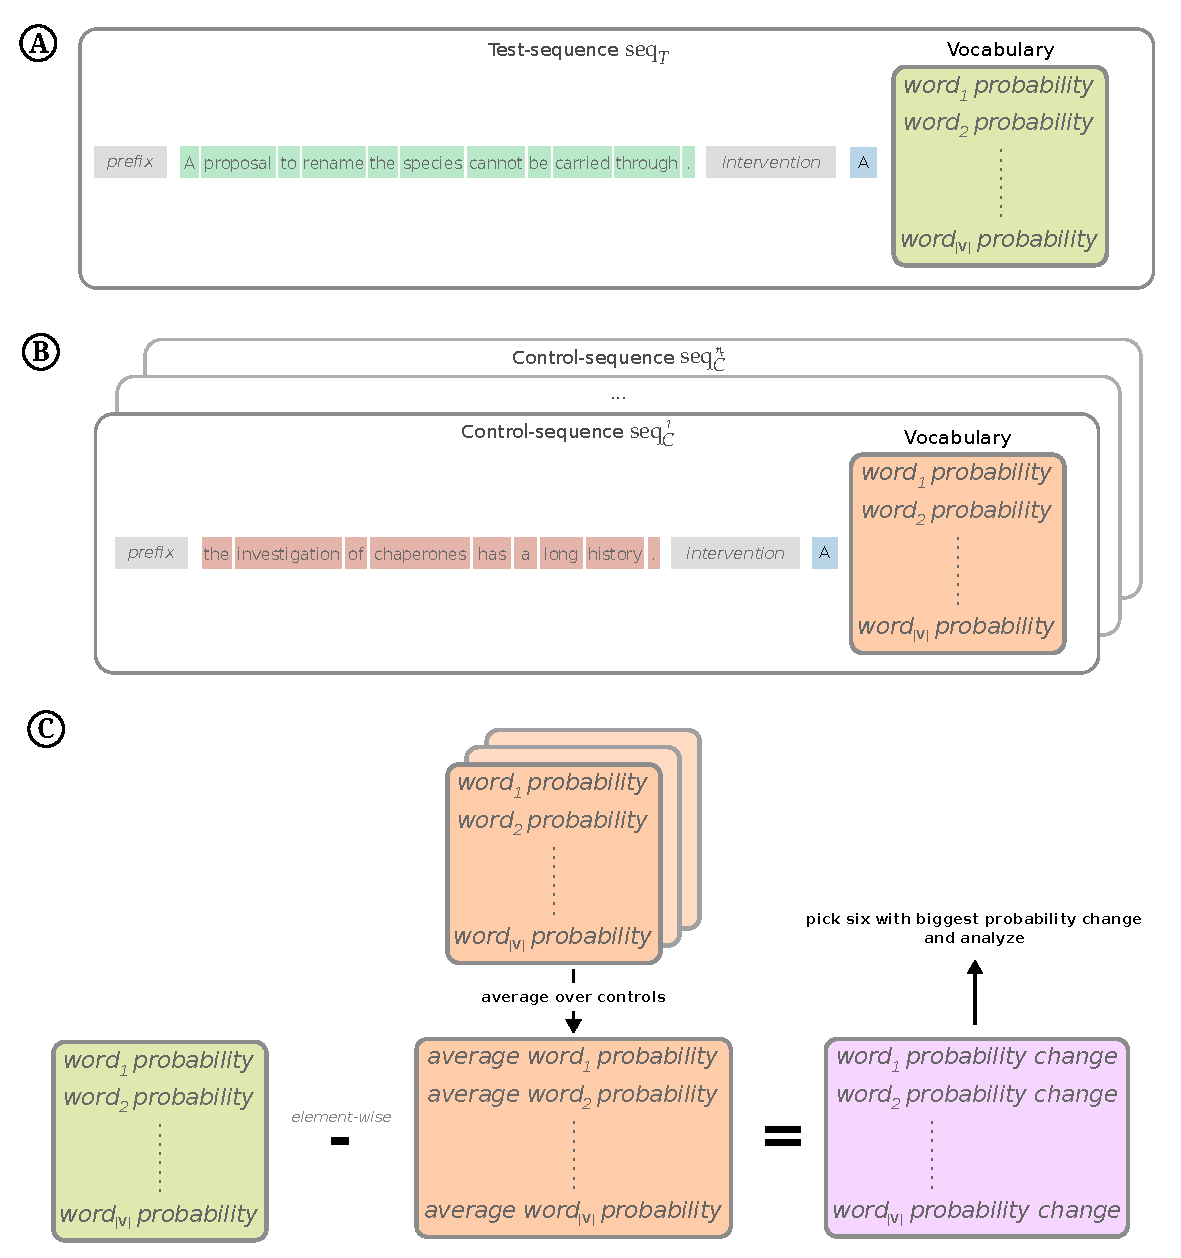
\includegraphics[width=\textwidth]{methods/prob_change_setup.pdf}
    \caption{Experimental setup for the probability change analysis. \textbf{A}: In the Test-sequence we record probabilities of all words within the vocabulary (green) after presentation of prefix (grey), encoding-sentence (green), intervention (grey) and the start of the test-sentence (blue). \textbf{B}: In the Control-sequences we record probabilities of all words within the vocabulary (orange) after presentation of prefix, control-sentence (red), intervention (grey) and the start of the test-sentence (blue). \textbf{C}: Probabilities of words from the Control-sequences are averaged, and then subtracted with the probabilities of the words from the Test-sequence to obtain the probability change for each word in the Vocabulary (purple). The six words which have the biggest positive probability change are analyzed.}
    \label{fig:prob_change_experiment}
\end{figure}

\subsubsection{Results}

\begin{table} \centering
\scalebox{0.9}{
\begin{tabular}{c c c c c c c c}
\hline
\multicolumn{8}{l}{{\cellcolor{gray!25}\small Sentence}}\\
\thead{target noun} & \thead{probability\\in test-\\sequence} & \thead{\#1} & \thead{\#2} & \thead{\#3} & \thead{\#4} & \thead{\#5} & \thead{\#6} \\
\hline\hline
\multicolumn{8}{p{1.08\linewidth}}{\cellcolor{gray!25}the section on current routes adds nothing to the info .}\\
\thead{\footnotesize section\\} &\thead{\footnotesize 0.629} & \colorbox[rgb]{0.59, 0.78, 0.64}{\thead{\footnotesize section\\(0.6284)}} & \colorbox[rgb]{1.0, 1.0, 0.0}{ \thead{\footnotesize paragraph\\(0.0131) \hfill}} & \colorbox[rgb]{1.0, 0.75, 0.0}{\thead{\footnotesize sections\\(0.012) \hfill}} & \colorbox[rgb]{1.0, 1.0, 0.0}{\thead{\footnotesize page\\(0.0089)}} & \colorbox[rgb]{1.0, 1.0, 0.0}{\thead{\footnotesize part\\(0.0079)}} &\colorbox[rgb]{0.6, 0.4, 0.8}{\thead{\footnotesize route\\(0.0077)}} \\
\hline
\multicolumn{8}{p{1.08\linewidth}}{\cellcolor{gray!25}the base of the buildings contains commercial space , including two restaurants , a dental office ( pinnacle dental ) , a medical clinic , and spa , while the surrounding area will consist of public parks , shops and recreation spaces .}\\
\thead{\footnotesize base\\} &\thead{\footnotesize 0.424} & \colorbox[rgb]{0.59, 0.78, 0.64}{\thead{\footnotesize base\\(0.4239)}} & \colorbox[rgb]{0.6, 0.4, 0.8}{\thead{\footnotesize building\\(0.0288)}} & \colorbox[rgb]{1.0, 0.75, 0.0}{\thead{ \footnotesize bases\\(0.017)}} &  \colorbox[rgb]{0.92, 0.3, 0.26}{\thead{\footnotesize location\\(0.0079)}} & \colorbox[rgb]{0.6, 0.4, 0.8}{\thead{\footnotesize area\\(0.0076)}} & \colorbox[rgb]{0.6, 0.4, 0.8}{\thead{\footnotesize buildings\\(0.0065)}} \\
\hline
\multicolumn{8}{p{1.08\linewidth}}{\cellcolor{gray!25}the genetic variation among the viruses isolated from different places ( 7-8 ) increases the difficulty of developing vaccines against it .}\\
\thead{\footnotesize variation\\} &\thead{\footnotesize 0.919} & \colorbox[rgb]{0.59, 0.78, 0.64}{\thead{\footnotesize variation\\(0.9169)}} & \colorbox[rgb]{1.0, 1.0, 0.0}{ \thead{\footnotesize variance\\(0.0229)}} & \colorbox[rgb]{1.0, 0.75, 0.0}{ \thead{\footnotesize variant\\(0.0135)}} & \colorbox[rgb]{1.0, 0.75, 0.0}{\thead{\footnotesize variations\\(0.0133)}} &  \colorbox[rgb]{1.0, 1.0, 0.0}{ \thead{\footnotesize variability\\(0.0083)}} & \colorbox[rgb]{1.0, 0.75, 0.0}{ \thead{\footnotesize variants\\(0.0009)}} \\
\hline
\multicolumn{8}{p{1.08\linewidth}}{\cellcolor{gray!25}the edwardian semi-detached houses of brantwood road , facing the park have an art deco style whilst those in ashburnham road include ornate balconies .   }\\
\thead{\footnotesize houses} & \thead{\footnotesize 0.95} & \colorbox[rgb]{0.59, 0.78, 0.64}{ \thead{\footnotesize houses\\(0.9498)}} & \colorbox[rgb]{1.0, 1.0, 0.0}{ \thead{\footnotesize homes\\(0.0092)}} & \colorbox[rgb]{1.0, 0.75, 0.0}{\thead{\footnotesize house\\(0.0076)}} & \colorbox[rgb]{1.0, 0.75, 0.0}{\thead{\footnotesize \_houses\\(0.0016)}} & \colorbox[rgb]{1.0, 1.0, 0.0}{\thead{\footnotesize dwellings\\(0.0016)}} & \colorbox[rgb]{1.0, 1.0, 0.0}{\thead{\footnotesize places\\(0.0006)}} \\
\hline
\multicolumn{8}{p{1.08\linewidth}}{\cellcolor{gray!25}for protestant denominations , the purposes of marriage include intimate companionship , rearing children and mutual support for both husband and wife to fulfill their life callings .}\\
\thead{\footnotesize purposes} & \thead{\footnotesize 0.855} &  \colorbox[rgb]{0.59, 0.78, 0.64}{\thead{\footnotesize purposes\\(0.8546)}} & \colorbox[rgb]{1.0, 0.75, 0.0}{ \thead{\footnotesize purpose\\(0.1033)}} & \colorbox[rgb]{1.0, 1.0, 0.0}{ \thead{\footnotesize uses\\(0.0035)}} & \colorbox[rgb]{0.92, 0.3, 0.26}{\thead{\footnotesize ends\\(0.0034)}} & \colorbox[rgb]{0.92, 0.3, 0.26}{\thead{\footnotesize means\\(0.0025)}} & \colorbox[rgb]{1.0, 1.0, 0.0}{\thead{\footnotesize functions\\(0.0016)}} \\
\hline
\end{tabular}
}
\caption{Example data of the words with the biggest change in the probability change experiment. For each sentence, the target word is provided together with the model's absolute probability for the target word given the repeat context. The rest of the columns denote the words with highest probability change. The probability change is in the brackets below the word. Words the transformer predicted to be a continuation without a blank-space start with ``\_''. Colors mark error categories of the error analysis: \textit{Green}: Verbatim repetition; \textit{Yellow}: Semantically correct, syntactically correct; \textit{Orange}: Semantically correct, syntactically incorrect;  \textit{Red}: Semantically incorrect, syntactically corrrect; \textit{Purple}: Position shifted word; Other categories did occur in this subset.} \label{Tab:prediction_change}
\end{table}
% TODO: !

The first ten results for the experiment can be found in Table \ref{Tab:prediction_change}.
A clear pattern for the word with the highest probability change can be seen. Consistent with the findings of the previous experiment, it is almost always the verbatim repetition of the appropriate word in the encoding-sentence.
To draw more conclusions, we categorize each word of the top six words with the biggest positive change into eight categories.
These categories are determined manually by us based on the relationship of the word to the encoding-sentence in the context.
For instance, given the Test-sequence "[\textit{prefix}] the investigation of chaperones has a long history . [\textit{intervention}] the investigation of chaperones [???]" the prediction ``has'' in the position [???] is the verbatim repetition of the previous context, and ``have'' would be semantically correct, but syntactically wrong (subject-verb-disagreement).
We use following categories:\\
\textbf{Verbatim repetition}
A word that is the verbatim repetition of the word in the encoding-sentence (e.g. ``has'').\\
\textbf{Semantically correct, syntactically correct}
A word that is semantically and syntactically fitting -- in other words, a good synonym.
This category only includes words that preserve the meaning of the sentence, and words which allow the sentence to be continued as given in the encoding sentence (e.g. ``carries'').\\
\textbf{Semantically correct, syntactically incorrect}
A word which may semantically fit, but is syntactically wrong given the encoding sentence. For instance ``have'' with wrong subject-verb-agreement or ``had'' having the wrong tense.\\
\textbf{Semantically incorrect, syntactically correct}
A word which semantically does not fit, but is within the same POS-category with the repeated word (e.g. ``belongs'').\\
\textbf{Semantically incorrect, syntactically incorrect)}
A word which neither matches semantically nor syntactically (e.g. ``proudly'').\\
\textbf{Position shifted word}
A word which is predicted at a wrong sequence position -- it originally appeared in a different position of the encoding-sentence as the repeated word (e.g. ``long'').\\
\textbf{Other}
All words which cannot be categorized in the categories above.
For example, these may are single letter predictions such as ``C'' or in rare cases words which have appeared in the intervention\footnote{This happened exactly six times, but only in the noun condition.}.\\

The result of the categorization can be seen in Table \ref{Tab:prediction_change_analysis}.
For each category, the cumulative probability change percentage of all words within the category is shown alongside with the absolute category probability change.
The probability change percentage is computed by adding the probability change of each word within the category, obtaining the absolute category probability change.
This value is divided by the sum of the absolute category probability change of all categories, resulting in the cumulative probability change percentage.

The results show that the transformer given the repeat sentence context shifts the probability distribution mostly towards the verbatim repeated word from the context.
For nouns $89.51\%$ of probability change happens within the \textit{verbatim repetition} category.
For verbs, this effect is by $5\%$ stronger with $94.26\%$.

To ease the interpretation of the results we group both \textit{semantically correct} (second and third) categories: their probability change percentage together is $5.22\%$ and $4.43\%$ for nouns and verbs respectively.
Moreover, we group both \textit{syntactically correct} (second and fourth) categories, together they have a probability change percentage of $3.03\%$ and $3.56$ for nouns and verbs respectively.

Occurrences of words within categories mainly happen for the first four categories.
This is more so the case for verbs than for nouns, where a respectable amount of word occurrences resides in the ``position shifted word'' category.
For verbs, most occurrences are in the \textit{semantically correct, syntactically incorrect}-category $132$ occurrences.
For nouns, the maximal occurrences are in the \textit{semantically correct, syntactically correct}-category with $82$ occurrences.
Note that for both nouns and verbs in $58$ of $60$ sentences the verbatim repetition was present.
In the case of nouns, these were two sentences in which the noun was the first word of the sentence.

The difference in probability change between nouns and verbs mainly stems from an increase in probability change in the ``verbatim repetition'' category for verbs compared to nouns and a reduction of probability change in the categories ``position shifted word'' and ``other''.
In the \textit{semantically correct, syntactically correct}-category the transformer shows a higher probability change percentage for verbs than for nouns.

\begin{table} \centering
\begin{threeparttable}
\begin{tabular}{l | c c | c c}
\toprule
{} & \multicolumn{2}{c|}{\thead{nouns}} & \multicolumn{2}{c}{\thead{verbs}} \\
\thead{word category} &  \thead{cumulative probability-\\change percentage\\(absolute)} & \thead{occurrences} & \thead{cumulative probability-\\change percentage \\(absolute)} &  \thead{occurrences} \\
\midrule
\thead{verbatim repetition}                              &   89.51 (37.31) & 58 &  94.26 (47.12)  &  58 \\
\thead{semantically correct,\\syntactically correct}     &     1.5 (0.62)  & 82 &   2.58 (1.29)   &  83 \\
\thead{semantically correct,\\syntactically incorrect}   &    3.72 (1.55)  & 80 &   1.85 (0.92)   & 132 \\
\thead{semantically incorrect,\\syntactically correct}   &    1.53 (0.63)  & 70 &   0.98 (0.49)   &  54 \\
\thead{semantically incorrect,\\syntactically incorrect} &    0.65 (0.27)  & 16 &   0.24 (0.12)   &  17 \\
\thead{position\\shifted word}                           &    1.74 (0.72)  & 39 &   0.08 (0.04)   &   4 \\
\thead{other}                                            &    1.36 (0.57)  & 15 &   0.02 (0.01)   &   3 \\
\bottomrule
\end{tabular}
\caption{Categorization of the six words with the highest probability change in each sequence for verbs and nouns. We show the cumulative probability change percentage for each word category, together with the summed probability change within the category in brackets. This allows us to see how much probability change happens for each category -- in other words, which categories are affected the most by the encoding sentence in the context. The "occurrences" column shows the amount of times a word of the respective category appears within the top six predictions. As these are chosen irrespective of their actual probability change, the number of occurences cannot be attributed much importance.} \label{Tab:prediction_change_analysis}
\end{threeparttable}
\end{table}

\subsubsection{Interim Discussion}

Consistent with the findings of the previous experiment the highest probability change happens within the \textit{verbatim repetition}-category.
Moreover we find that the grouped \textit{semantically correct} categories have a .
The word-semantic copy-paste fWM M3 sets forth that synonyms of the continued word of the matched previous context are predicted.
Synonyms are semantically correct words independent of their syntactical correctness.
Hence, predictions within the \textit{semantically correct} categories are consistent with a word-semantic copy-paste fWM as posited in M3.
We can see that the second highest proportion of probability change just happens within these categories.
This further reinforces our previous discussion that a word-semantic copy paste fWM such as M3 approximates the transformers' fWM well.
Moreover, this confirms our prior hypothesis that we may have not probed the right subset of synonyms:
Although repeat surprisal in the syntactic word swap condition SYN of the previous experiment \ref{ex:2_word_swap_results} was close to $100\%$ and thus did not allow for a conclusive judgement, this experiment shows that $4.43\%$ of probability change lies within the \textit{semantically correct} category.
For that reason, the word-semantic copy paste fWM seems to approximate computational operations of transformer fWM for both nouns and verbs.

At a first glance, the probability change in the \textit{syntactically correct} categories would then by analogy hint towards a lexical-syntactic copy paste fWM M1.
In M1 probability is put into words which are within the same POS-category as the continued word of prior context.
But a lexical-syntactic copy paste mechanism would be expected to spread its probabilities over all or large proportion of words within a POS-category, and not a small subset.
The results of the within-POS-category word-swap condition ARB in the previous experiment \ref{ex:2_word_swap_results} show that the contrary is the case: in most cases the transformer fWM reduces the probability of words which are syntactically related, but semantically unrelated.
That does not mean that this happens for every word, which also can be seen in the previous experiment.
Thus, these results do not speak against the preliminary conclusions of the previous discussion, in which the lexical-syntactic copy-paste fWM was deemed to not approximate transformer fWM well.

An interesting observation concerns the difference in probability change percentages for nouns and verbs, especially when taking into account the amount of occurrences for each category.
Noticeably, in the \textit{semantically correct, syntactically incorrect}-category there are more occurrences for verbs, but a smaller probability change percentage than for nouns.
Analysis shows that these occurrences are mostly inflections of the verb (e.g. given "add", the inflections ``adds'' or ``added''). Their probability change percentage is so low, because they usually only occur when the model puts most of the probability change into the verbatim repeated word, without putting probability change into other synonyms.

Another observation is that probability change for the \textit{position shifted word} is almost only present for nouns.
This could be due to the much bigger availability of nouns within a sentence:
whereas our test sentence only have 1-2 verbs, they normally include multiple other nouns.
Thus there is just a higher amount of words the transformer fWM can confounded with the continued word of the matched prior context.

\newpage
